\documentclass[12pt,a4paper,oneside]{report}
% Preámbulo compartido — Informe Técnico Scapegoat Tree
\usepackage[utf8]{inputenc}
\usepackage[T1]{fontenc}
\usepackage[spanish,es-tabla]{babel}
\usepackage{mathptmx}
\usepackage{textcomp}
\usepackage{microtype}
\usepackage{geometry}
\usepackage[dvipsnames]{xcolor}
\usepackage{graphicx}
\usepackage{booktabs}
\usepackage{longtable}
\usepackage{array}
\usepackage{multirow}
\usepackage{caption}
\usepackage{subcaption}
\usepackage{float}
\usepackage{amsmath,amssymb,amsthm}
\usepackage{mathtools}
\usepackage{listings}
\usepackage{fancyhdr}
\usepackage{titlesec}
\usepackage{enumitem}
\usepackage{tikz}
\usepackage{pgfplots}
\usetikzlibrary{arrows.meta,positioning,shapes.geometric,fit,backgrounds,calc}

\pgfplotsset{compat=1.18}

\geometry{left=3cm, right=2.5cm, top=2.8cm, bottom=2.8cm}
\setlength{\parskip}{0.45em}
\setlength{\parindent}{1.2em}
\linespread{1.15}

\definecolor{codebg}{RGB}{244,246,248}
\definecolor{codeframe}{RGB}{49,87,213}
\definecolor{esanblue}{RGB}{26,26,46}

% Lenguaje Go para listings (no viene por defecto)
\lstdefinelanguage{Go}{
  morekeywords={break,case,chan,const,continue,default,defer,else,fallthrough,for,func,go,goto,if,import,interface,map,package,range,return,select,struct,switch,type,var,bool,byte,complex64,complex128,error,float32,float64,int,int8,int16,int32,int64,rune,string,uint,uint8,uint16,uint32,uint64,uintptr,true,false,nil},
  sensitive=true,
  morecomment=[l]{//},
  morecomment=[s]{/*}{*/},
  morestring=[b]",
  morestring=[b]',
}

\lstdefinestyle{goi}{
  basicstyle=\ttfamily\footnotesize,
  breaklines=false,
  columns=fullflexible,
  keepspaces=true,
  showstringspaces=false,
}

% Código inline Go con caracteres especiales (genéricos, llaves, etc.)
\newcommand{\go}[1]{\lstinline[style=goi]|#1|}

\lstdefinestyle{gocode}{
  language=Go,
  basicstyle=\ttfamily\footnotesize,
  keywordstyle=\color{blue}\bfseries,
  commentstyle=\color{gray}\itshape,
  stringstyle=\color{teal},
  numbers=left,
  numberstyle=\tiny\color{gray},
  stepnumber=1,
  numbersep=8pt,
  backgroundcolor=\color{codebg},
  frame=single,
  rulecolor=\color{codeframe},
  breaklines=true,
  tabsize=4,
  showstringspaces=false,
  literate={á}{{\'a}}1 {é}{{\'e}}1 {í}{{\'i}}1 {ó}{{\'o}}1 {ú}{{\'u}}1
           {ñ}{{\~n}}1 {Á}{{\'A}}1 {É}{{\'E}}1 {Í}{{\'I}}1 {Ó}{{\'O}}1 {Ú}{{\'U}}1 {Ñ}{{\~N}}1
}

\lstdefinestyle{sqlcode}{
  language=SQL,
  basicstyle=\ttfamily\footnotesize,
  backgroundcolor=\color{codebg},
  frame=single,
  rulecolor=\color{codeframe},
  breaklines=true
}

\lstdefinestyle{jsoncode}{
  basicstyle=\ttfamily\footnotesize,
  backgroundcolor=\color{codebg},
  frame=single,
  rulecolor=\color{codeframe},
  breaklines=true
}

\lstdefinestyle{pscode}{
  basicstyle=\ttfamily\footnotesize,
  backgroundcolor=\color{codebg},
  frame=single,
  rulecolor=\color{codeframe},
  breaklines=true,
  literate={\$}{{\$}}1
}

\captionsetup{
  font=small,
  labelfont=bf,
  justification=centering,
  skip=8pt
}

\captionsetup[lstlisting]{singlelinecheck=false}

\setlength{\headheight}{15pt}
\pagestyle{fancy}
\fancyhf{}
\fancyhead[L]{\small\textit{Algoritmos y Estructura de Datos --- ESAN 2026-1}}
\fancyhead[R]{\small\textit{Scapegoat Tree}}
\fancyfoot[C]{\thepage}
\renewcommand{\headrulewidth}{0.4pt}

\titleformat{\chapter}[display]
  {\normalfont\bfseries\color{esanblue}}
  {\chaptertitlename\ \thechapter}{12pt}{\Large}
\titlespacing*{\chapter}{0pt}{-10pt}{20pt}

\titleformat{\section}{\normalfont\bfseries\color{esanblue}}{\thesection}{0.8em}{}
\titleformat{\subsection}{\normalfont\bfseries}{\thesubsection}{0.8em}{}

\newtheorem{teorema}{Teorema}[chapter]
\newtheorem{invariante}[teorema]{Invariante}

\newcommand{\bigO}{\mathcal{O}}
\newcommand{\Scapegoat}{\textit{Scapegoat Tree}}

% hyperref al final del preámbulo
\usepackage{hyperref}
\usepackage{bookmark}

\hypersetup{
  colorlinks=true,
  linkcolor=NavyBlue,
  citecolor=NavyBlue,
  urlcolor=NavyBlue,
  pdftitle={Informe Tecnico --- Scapegoat Tree},
  pdfauthor={Universidad ESAN}
}


\begin{document}

%==============================================================================
% PORTADA
%==============================================================================
\begin{titlepage}
  \thispagestyle{empty}
  \centering
  \vspace*{1.2cm}
  {\large\textbf{UNIVERSIDAD ESAN}\par}
  \vspace{0.3cm}
  {\normalsize Facultad de Ciencias de la Computación\par}
  \vspace{2.2cm}
  {\huge\bfseries\color{esanblue} INFORME TÉCNICO FINAL\par}
  \vspace{1.2cm}
  {\Large Estudio, implementación, integración con base de datos\\[0.35em]
  y simulación visual del \Scapegoat\par}
  \vspace{2cm}
  \begin{tabular}{@{}p{4.2cm}p{9.2cm}@{}}
    \toprule
    \textbf{Curso} & Algoritmos y Estructura de Datos (2026-1) \\
    \textbf{Docente} & Marks Calderón Niquin \\
    \textbf{Integrantes} & [Nombre Apellido --- Código] \\
    & [Nombre Apellido --- Código] \\
    \textbf{Repositorio} & \url{https://github.com/Fravely/Spacegoat-tree} \\
    \textbf{Base de datos} & Microsoft SQL Server (\texttt{go-mssqldb}) \\
    \textbf{Implementación} & Go 1.23 \textbullet{} Vue.js 3 \\
    \textbf{Fecha} & Junio 2026 \\
    \bottomrule
  \end{tabular}
  \vfill
  {\small Trabajo Final --- Semestre Académico 2026-1\par}
\end{titlepage}

\pagenumbering{roman}
\chapter*{Resumen}
\phantomsection
\addcontentsline{toc}{chapter}{Resumen}

El presente informe documenta el estudio, diseño e implementación del \textbf{\Scapegoat}, estructura de datos de búsqueda balanceada propuesta por Galperin y Rivest (1993), en el marco del curso de Algoritmos y Estructura de Datos de la Universidad ESAN. A diferencia de los árboles AVL o Red-Black, esta estructura restaura el balance mediante la reconstrucción completa de subárboles desbalanceados ---seleccionando un nodo \textit{scapegoat}--- en lugar de aplicar rotaciones locales ni almacenar metadatos de balance por nodo.

El trabajo comprende cuatro componentes integrados: un paquete genérico en Go (\texttt{scapegoat/}) con operaciones de inserción, búsqueda, eliminación y trazabilidad algorítmica; una capa de persistencia sobre SQL Server; una API REST que sincroniza la base de datos con el índice en memoria; y una interfaz Vue.js que visualiza el árbol y anima el proceso de reconstrucción. Las pruebas unitarias, los benchmarks y la comparación contra un \texttt{map} de referencia validan el comportamiento esperado. Los resultados experimentales confirman que las inserciones ordenadas provocan reconstrucciones frecuentes, mientras que la búsqueda mantiene tiempos estables del orden de 214~ns/op con $n = 10^5$ nodos.

\vspace{0.8em}
\noindent\textbf{Palabras clave:} Scapegoat Tree, árbol binario de búsqueda, balance por reconstrucción, Go, SQL Server, complejidad amortizada, estructuras de datos.

\tableofcontents
\listoffigures
\listoftables

\pagenumbering{arabic}

\chapter{Introducción y marco teórico}

\section{Contexto del problema computacional}

Los árboles binarios de búsqueda (BST, \textit{Binary Search Tree}) constituyen una de las estructuras más didácticas y, al mismo tiempo, más traicioneras de la computación moderna. Su invariante es elegante: para todo nodo $u$, las claves del subárbol izquierdo son menores que $\mathrm{key}(u)$ y las del subárbol derecho son mayores. Esa propiedad habilita búsquedas que, en el caso ideal, descienden por la altura del árbol en tiempo $\bigO(\log n)$.

El problema aparece cuando la secuencia de inserciones no es aleatoria. Insertar claves ordenadas $1, 2, 3, \ldots, n$ produce un árbol degenerado: una lista enlazada disfrazada de árbol. La altura pasa a ser $n-1$ y cada búsqueda cuesta $\bigO(n)$. Durante décadas, la respuesta dominante fue introducir \textbf{factores de balance} en cada nodo (AVL, Red-Black) y corregir desviaciones mediante \textbf{rotaciones locales}.

En 1993, Galperin y Rivest propusieron un enfoque radicalmente distinto en su artículo \textit{Scapegoat Trees}. En lugar de mantener balance incremental con rotaciones, permiten que el árbol se desbalancee temporalmente y, cuando la profundidad excede un umbral teórico, identifican un nodo \textbf{scapegoat} (chivo expiatorio) cuyo subárbol se \textbf{reconstruye completamente} en orden balanceado. No hay rotaciones. No hay campos de balance por nodo. El precio se paga en reconstrucciones que pueden tocar $\bigO(n)$ nodos en una operación aislada, pero cuyo costo \textbf{amortizado} permanece logarítmico bajo distribuciones razonables de operaciones.

Este informe documenta la implementación completa de esa estructura en Go, su integración con SQL Server como capa de persistencia, la exposición de una API REST para mutaciones y consultas, y una interfaz Vue.js que visualiza el comportamiento del algoritmo ---incluyendo la selección del scapegoat y la reconstrucción del subárbol--- en tiempo casi real.

\section{El paper de Galperin y Rivest (1993)}

\subsection{Problema fundacional}

En la década de 1990, las estructuras balanceadas dominantes (AVL, Red-Black, B-Trees) habían madurado, pero compartían una característica: \textbf{cada nodo almacena información adicional} para decidir cuándo y cómo rotar. Galperin y Rivest se preguntaron si era posible obtener altura $\bigO(\log n)$ amortizada \textbf{sin} almacenar metadatos de balance en los nodos y \textbf{sin} rotaciones.

\subsection{Definición formal}

Sea $T$ un \Scapegoat{} parametrizado por $\alpha \in (0.5, 1)$. El árbol mantiene dos contadores globales:

\begin{table}[H]
  \centering
  \caption{Contadores del algoritmo Scapegoat}
  \begin{tabular}{@{}cl@{}}
    \toprule
    \textbf{Símbolo} & \textbf{Definición} \\
    \midrule
    $n$ & Número actual de nodos \\
    $q$ & Máximo valor de $n$ alcanzado desde la última reconstrucción global \\
    \bottomrule
  \end{tabular}
\end{table}

La \textbf{profundidad máxima permitida} tras una inserción, dado el valor actual de $q$, es:
\begin{equation}
  d_{\max}(q) = \left\lfloor \log_{1/\alpha}(q) \right\rfloor
  \label{eq:dmax}
\end{equation}

Cuando la profundidad del nodo recién insertado supera $d_{\max}(q)$, el algoritmo asciende por el \textbf{camino de inserción} desde la hoja hacia la raíz buscando el nodo padre $p$ tal que:
\begin{equation}
  \mathrm{size}(\mathrm{hijo}) > \alpha \cdot \mathrm{size}(p)
  \label{eq:scapegoat-cond}
\end{equation}

donde $\mathrm{size}(u)$ denota el número de nodos en el subárbol raíz en $u$. Ese padre $p$ es el \textbf{scapegoat}. Su subárbol completo se aplana mediante un recorrido in-order, se almacena en un arreglo temporal y se reconstruye como un BST \textbf{perfectamente balanceado} seleccionando el elemento medio como raíz del subárbol.

Para la eliminación, el paper adopta una política más drástica: \textbf{no} se buscan scapegoats. Si tras eliminar un nodo se cumple:
\begin{equation}
  n < \alpha \cdot q
  \label{eq:global-rebuild}
\end{equation}
entonces se reconstruye \textbf{todo el árbol} y se asigna $q \leftarrow n$.

\subsection{Diagrama del algoritmo de inserción}

\begin{figure}[H]
  \centering
  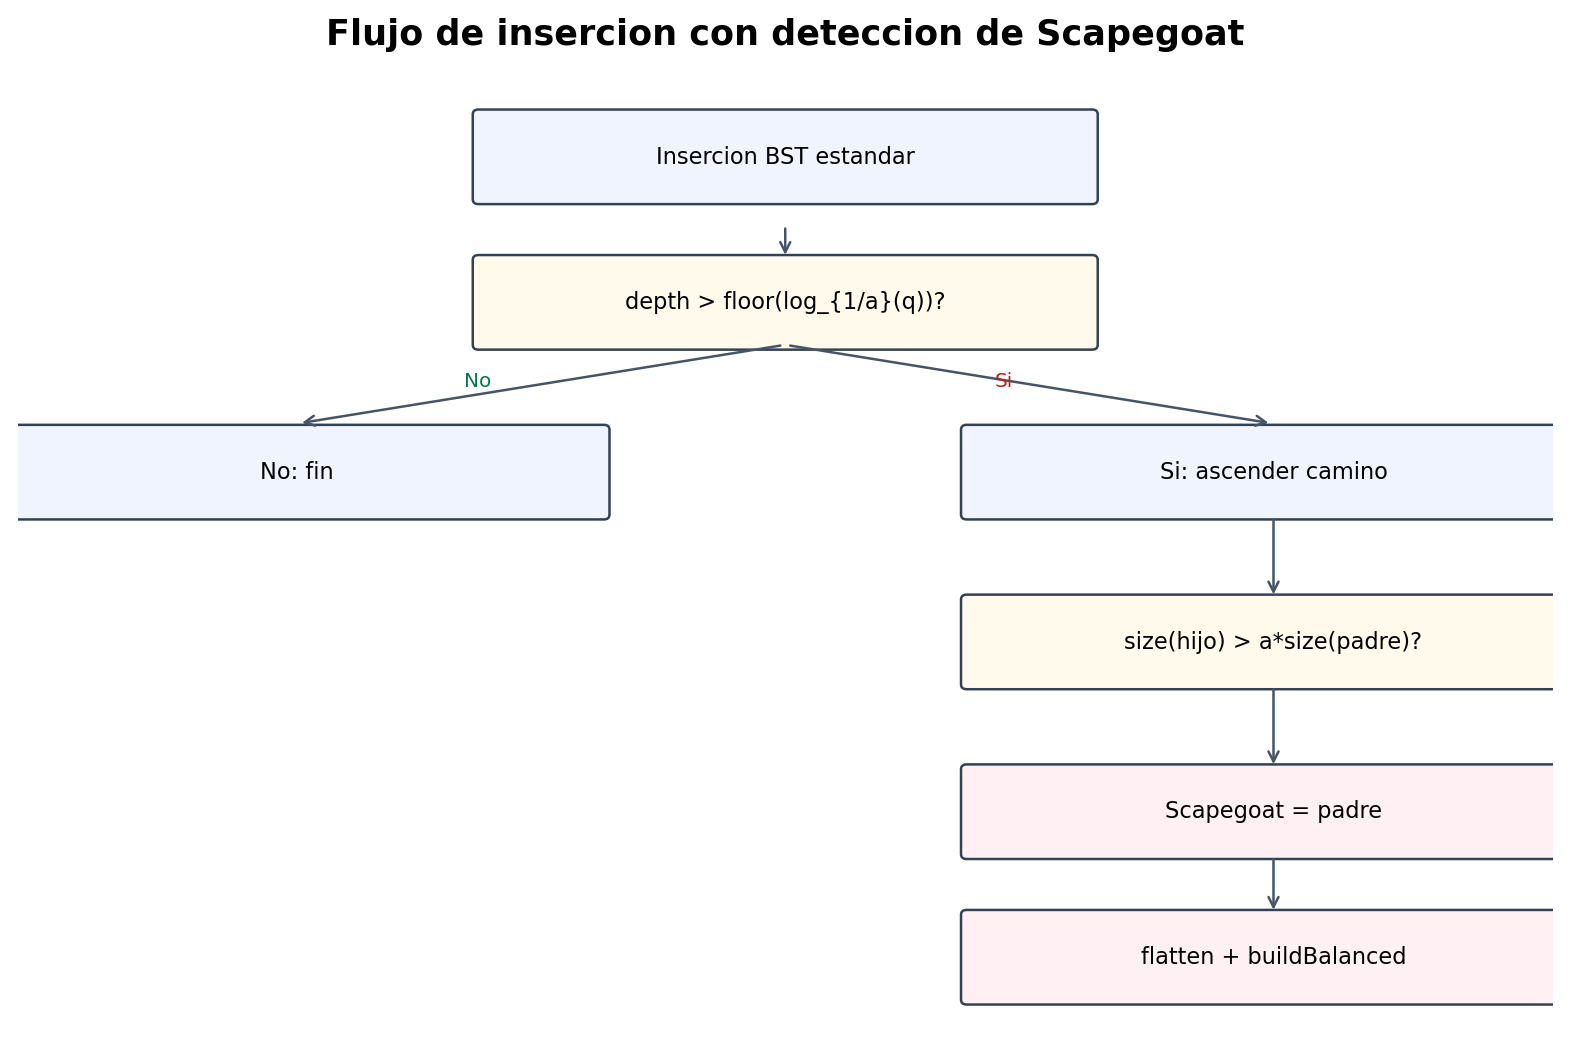
\includegraphics[width=0.92\textwidth]{diagrams/02-flujo-insercion.png}
  \caption{Flujo de inserción con detección de Scapegoat}
  \label{fig:flujo-insercion}
\end{figure}

\begin{figure}[H]
  \centering
  \begin{tikzpicture}[
    node distance=0.55cm and 1.1cm,
    startstop/.style={rectangle, rounded corners, draw=esanblue, fill=blue!8, minimum width=2.8cm, align=center, font=\small},
    decision/.style={diamond, draw=orange!70!black, fill=orange!10, aspect=2, inner sep=1pt, align=center, font=\footnotesize},
    arrow/.style={-{Stealth[length=2mm]}, thick}
  ]
    \node[startstop] (a) {Insertar clave $k$};
    \node[decision, below=of a] (b) {¿Árbol vacío?};
    \node[startstop, below left=0.9cm and 1.4cm of b] (c) {Crear raíz\\$n{=}1$, $q{=}1$};
    \node[startstop, below right=0.9cm and 1.4cm of b] (d) {Descender BST};
    \node[decision, below=of d] (e) {¿$\mathrm{depth} > d_{\max}(q)$?};
    \node[startstop, below left=of e] (f) {Fin};
    \node[startstop, below right=of e] (g) {Buscar scapegoat\\rebuild subárbol};
    \draw[arrow] (a) -- (b);
    \draw[arrow] (b) -- node[left, font=\scriptsize]{Sí} (c);
    \draw[arrow] (b) -- node[right, font=\scriptsize]{No} (d);
    \draw[arrow] (d) -- (e);
    \draw[arrow] (e) -- node[left, font=\scriptsize]{No} (f);
    \draw[arrow] (e) -- node[right, font=\scriptsize]{Sí} (g);
  \end{tikzpicture}
  \caption{Representación esquemática TikZ del algoritmo de inserción}
  \label{fig:tikz-insercion}
\end{figure}

\subsection{Invariantes y teoremas}

\begin{invariante}[Altura débil]
Mientras $n \geq \alpha \cdot q$ o tras una reconstrucción global, la altura del árbol está acotada por $d_{\max}(q) + \bigO(1)$.
\end{invariante}

\begin{teorema}[Galperin \& Rivest]
Una secuencia de $m$ operaciones de inserción y eliminación sobre un \Scapegoat{} con parámetro $\alpha$ tiene costo total $\bigO(m \log n)$, siendo el costo amortizado por operación $\bigO(\log n)$.
\end{teorema}

\section{Justificación frente a alternativas}

\begin{table}[H]
  \centering
  \caption{Comparación con AVL y Red-Black}
  \begin{tabular}{@{}lcc@{}}
    \toprule
    \textbf{Criterio} & \textbf{AVL / Red-Black} & \textbf{Scapegoat Tree} \\
    \midrule
    Metadato por nodo & Factor de balance o color & Ninguno \\
    Mecanismo de balance & Rotaciones locales & Reconstrucción de subárbol \\
    Peor operación individual & $\bigO(\log n)$ & $\bigO(n)$ \\
    Amortizado & $\bigO(\log n)$ & $\bigO(\log n)$ \\
    Complejidad de código & Alta & Media \\
    \bottomrule
  \end{tabular}
\end{table}

Frente al \texttt{map} nativo de Go, que ofrece $\bigO(1)$ amortizado pero no mantiene orden, el \Scapegoat{} expone \texttt{InOrder()} en $\bigO(n)$ y preserva la topología BST para fines pedagógicos. Frente a Skip Lists, nuestra elección es \textbf{determinista}, lo que simplifica pruebas y simulación visual.

\chapter{Arquitectura del sistema y lógica del código (backend en Go)}

\section{Filosofía de diseño}

El proyecto se organiza en cuatro capas desacopladas. La Figura~\ref{fig:arquitectura} resume la arquitectura; el paquete \texttt{scapegoat} no importa \texttt{database}, \texttt{net/http} ni persistencia, lo que permite ejecutar \texttt{go test ./scapegoat/...} de forma aislada.

\begin{figure}[H]
  \centering
  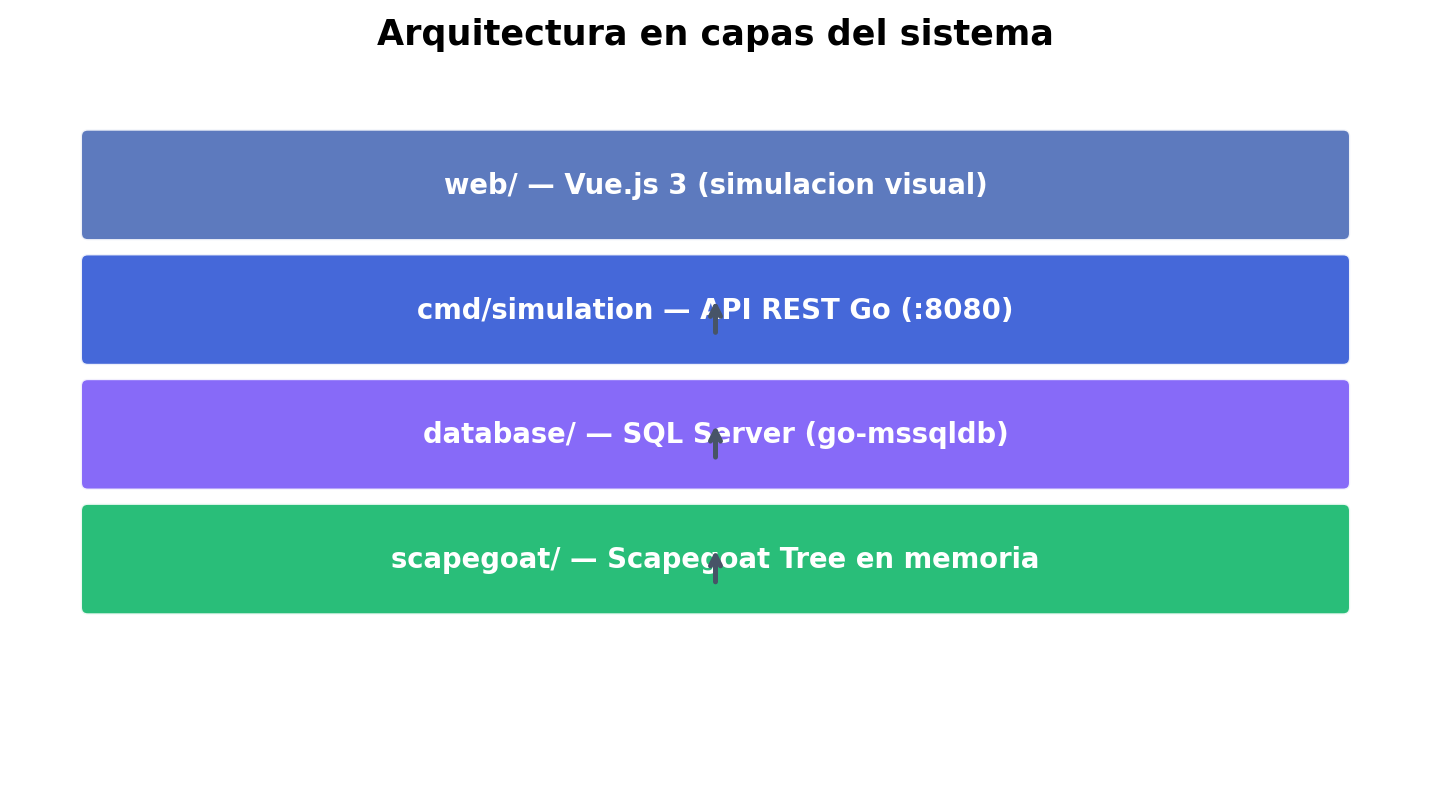
\includegraphics[width=0.88\textwidth]{diagrams/01-arquitectura.png}
  \caption{Arquitectura en capas del sistema}
  \label{fig:arquitectura}
\end{figure}

Go 1.18+ habilita \textbf{genéricos}. Usamos \go{Tree[K, V any]} con comparador externo, \go{NewOrdered[K Ordered, V any]} para tipos ordenados, y punteros \go{*node[K,V]} para hijos izquierdo y derecho.

\section{Tipos y estructuras de datos}

\subsection{Nodo interno}

\begin{lstlisting}[style=gocode,caption={Estructura de nodo interno},label={lst:node}]
type node[K, V any] struct {
    key         K
    value       V
    left, right *node[K, V]
}
\end{lstlisting}

\subsection{Árbol público}

\begin{lstlisting}[style=gocode,caption={Estructura Tree con contadores n, q y alpha},label={lst:tree}]
type Tree[K, V any] struct {
    root         *node[K, V]
    less         func(K, K) bool
    alpha        float64
    n, q         int
    rebuilds     int
    rebuiltNodes int
}
\end{lstlisting}

\begin{table}[H]
  \centering
  \caption{Campos de la estructura \texttt{Tree}}
  \begin{tabular}{@{}lp{9cm}@{}}
    \toprule
    \textbf{Campo} & \textbf{Rol} \\
    \midrule
    \texttt{root} & Puntero a la raíz; \texttt{nil} si el árbol está vacío \\
    \texttt{less} & Relación de orden estricto: \texttt{less(a,b)} $\Leftrightarrow$ $a < b$ \\
    \texttt{alpha} & Parámetro de balance $\alpha \in (0.5, 1)$ \\
    \texttt{n}, \texttt{q} & Contadores de nodos actuales y máximo desde última rebuild global \\
    \texttt{rebuilds} & Número de reconstrucciones realizadas \\
    \bottomrule
  \end{tabular}
\end{table}

\section{Catálogo de funciones principales}

\subsection{Constructores}

\go{New[K,V](alpha, less)} valida $\alpha \in (0.5, 1)$ y que \texttt{less} no sea \texttt{nil}. \texttt{NewOrdered} inyecta \go{less = func(a,b) bool { return a < b }}.

\subsection{Búsqueda e inserción}

\texttt{Search(key)} realiza búsqueda BST iterativa en $\bigO(h)$ donde $h$ es la altura. \texttt{Insert} y \texttt{InsertWithTrace} delegan en \texttt{insert}, que:
\begin{enumerate}[noitemsep]
  \item Inserta como BST ordinario.
  \item Incrementa $n$ y $q$ si la clave es nueva.
  \item Si $\mathrm{depth} > d_{\max}(q)$, asciende el camino buscando el scapegoat (Ec.~\ref{eq:scapegoat-cond}).
  \item Reconstruye el subárbol con \texttt{flatten} + \texttt{buildBalanced}.
\end{enumerate}

\subsection{Eliminación}

\texttt{Delete(key)} aplica eliminación BST clásica (tres casos). Si $n < \alpha \cdot q$, ejecuta reconstrucción global (Ec.~\ref{eq:global-rebuild}).

\subsection{Detección del scapegoat}

\begin{lstlisting}[style=gocode,caption={Fragmento de detección de scapegoat en inserción},label={lst:scapegoat}]
if depth > t.maxDepth(t.q) {
    for i := len(path) - 2; i >= 0; i-- {
        parent, child := path[i], path[i+1]
        if float64(size(child)) > t.alpha*float64(size(parent)) {
            scapegoatKey := parent.key
            trace.Scapegoat = &scapegoatKey
            flattenKeys(parent, &trace.RebuiltKeys)
            rebuilt := t.rebuild(parent)
            // Reenlazar rebuilt en el arbol...
            break
        }
    }
}
\end{lstlisting}

\subsection{Reconstrucción balanceada}

\begin{equation}
  d_{\max} = \left\lfloor \frac{\ln q}{\ln (1/\alpha)} \right\rfloor
\end{equation}

\texttt{rebuild(root)} aplana el subárbol in-order, incrementa contadores y llama \texttt{buildBalanced}, que selecciona el nodo medio garantizando altura $\lfloor \log_2 k \rfloor$ para $k$ nodos.

\begin{figure}[H]
  \centering
  \begin{tikzpicture}[
    box/.style={rectangle, draw, rounded corners, minimum width=2.2cm, minimum height=0.8cm, align=center, font=\small},
    arrow/.style={-{Stealth[length=2mm]}, thick}
  ]
    \node[box, fill=red!8] (a) {Subárbol desbalanceado};
    \node[box, fill=yellow!12, right=1.6cm of a] (b) {flatten in-order};
    \node[box, fill=yellow!12, right=1.2cm of b] (c) {buildBalanced};
    \node[box, fill=green!10, right=1.6cm of c] (d) {Subárbol balanceado};
    \draw[arrow] (a) -- (b);
    \draw[arrow] (b) -- (c);
    \draw[arrow] (c) -- (d);
  \end{tikzpicture}
  \caption{Proceso de reconstrucción (\texttt{rebuild})}
  \label{fig:rebuild}
\end{figure}

\section{Desafíos técnicos}

El cálculo de \texttt{size(u)} sin campo almacenado eleva el costo de detección. Con $n=1000$ e inserciones ordenadas observamos 375 reconstrucciones y 9762 nodos reconstruidos acumulados. La concurrencia se resuelve con \texttt{sync.Mutex} en la capa HTTP, no dentro del paquete \texttt{scapegoat}.

\chapter{Integración con la base de datos real}

\section{Modelo de datos}

La base de datos \texttt{InventarioProductosDB} contiene la tabla \texttt{dbo.Productos}:

\begin{table}[H]
  \centering
  \caption{Esquema relacional \texttt{dbo.Productos}}
  \begin{tabular}{@{}lll@{}}
    \toprule
    \textbf{Columna} & \textbf{Tipo} & \textbf{Restricción} \\
    \midrule
    \texttt{id} & \texttt{INT} & \texttt{PRIMARY KEY} \\
    \texttt{nombre} & \texttt{NVARCHAR(120)} & \texttt{NOT NULL} \\
    \texttt{categoria} & \texttt{NVARCHAR(80)} & \texttt{NOT NULL} \\
    \texttt{precio} & \texttt{DECIMAL(10,2)} & \texttt{NOT NULL} \\
    \texttt{stock} & \texttt{INT} & \texttt{NOT NULL} \\
    \bottomrule
  \end{tabular}
\end{table}

\begin{lstlisting}[style=gocode,caption={Struct Go \texttt{Product}},label={lst:product}]
type Product struct {
    ID       int
    Name     string
    Category string
    Price    float64
    Stock    int
}
\end{lstlisting}

\section{Conexión Go $\leftrightarrow$ SQL Server}

Driver: \texttt{github.com/denisenkom/go-mssqldb}. Configuración vía variables de entorno (\texttt{SQLSERVER\_HOST}, \texttt{SQLSERVER\_DATABASE}, etc.) o \texttt{SQLSERVER\_DSN}. Pool: \texttt{MaxOpenConns(5)}, \texttt{ConnMaxIdleConns(5)}, timeout de 10~s en \texttt{PingContext}.

\section{Estrategia de carga}

\begin{enumerate}
  \item \texttt{ListProducts(ctx, db)} $\rightarrow$ \texttt{SELECT ... ORDER BY id}.
  \item Para cada \texttt{Product}: \texttt{tree.Insert(product.ID, product)}.
\end{enumerate}

\begin{lstlisting}[style=gocode,caption={Carga de productos al índice en memoria}]
for _, product := range products {
    index.Insert(product.ID, product)
}
\end{lstlisting}

\section{Rol del \Scapegoat{} sobre datos persistidos}

SQL Server resuelve persistencia; el \Scapegoat{} en RAM actúa como \textbf{índice ordenado por \texttt{id}} con búsqueda $\bigO(\log n)$ amortizada y recorrido \texttt{InOrder()} en $\bigO(n)$.

\begin{figure}[H]
  \centering
  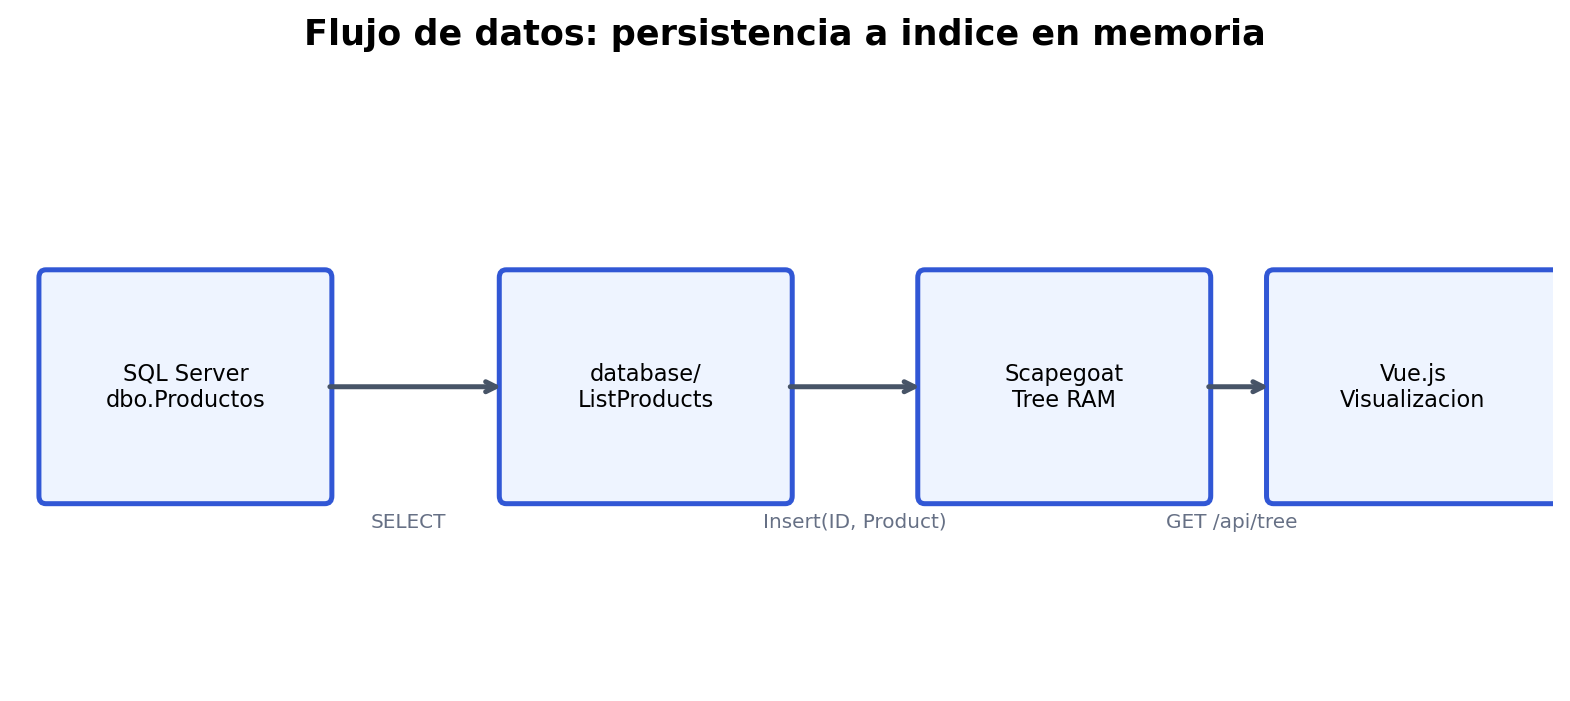
\includegraphics[width=0.92\textwidth]{diagrams/03-flujo-datos.png}
  \caption{Flujo de datos desde SQL Server al índice en memoria}
  \label{fig:flujo-datos}
\end{figure}

\begin{figure}[H]
  \centering
  \begin{tikzpicture}[
    actor/.style={rectangle, draw, rounded corners, minimum width=2cm, minimum height=0.7cm, align=center, font=\footnotesize},
    arrow/.style={-{Stealth[length=2mm]}, thick}
  ]
    \node[actor] (ss) {SQL Server};
    \node[actor, right=1.2cm of ss] (db) {database/};
    \node[actor, right=1.2cm of db] (api) {API Go};
    \node[actor, right=1.2cm of api] (st) {Scapegoat};
    \node[actor, right=1.2cm of st] (ui) {Vue.js};
    \draw[arrow] (ss) -- node[above] {SELECT} (db);
    \draw[arrow] (db) -- node[above] {[]Product} (api);
    \draw[arrow] (api) -- node[above] {Insert} (st);
    \draw[arrow] (st) -- node[above] {JSON} (ui);
  \end{tikzpicture}
  \caption{Secuencia de integración con base de datos}
  \label{fig:seq-db}
\end{figure}

\chapter{Diseño de la API REST (Go)}

El servidor en \go{cmd/simulation/main.go} expone los endpoints sobre \go{http.ListenAndServe(":8080", mux)}.

\begin{table}[H]
  \centering
  \caption{Endpoints de la API REST}
  \begin{tabular}{@{}llp{6.5cm}@{}}
    \toprule
    \textbf{Método} & \textbf{Ruta} & \textbf{Descripción} \\
    \midrule
    GET & \texttt{/api/tree} & Estado del árbol, métricas e \texttt{inOrder} \\
    POST & \texttt{/api/products} & Insertar o actualizar producto \\
    GET & \texttt{/api/products/\{id\}} & Búsqueda por ID en el árbol \\
    DELETE & \texttt{/api/products/\{id\}} & Eliminar producto \\
    POST & \texttt{/api/reset} & Reiniciar dataset semilla \\
    \bottomrule
  \end{tabular}
\end{table}

\section{Ejemplo de respuesta con traza}

\begin{lstlisting}[style=jsoncode,caption={Fragmento de respuesta POST /api/products}]
{
  "message": "Producto 109 insertado",
  "trace": {
    "path": [105, 109],
    "inserted": true,
    "depth": 1,
    "maxDepth": 3,
    "scapegoat": null,
    "rebuiltKeys": []
  }
}
\end{lstlisting}

\section{Sincronización y concurrencia}

\begin{lstlisting}[style=gocode,caption={Estado compartido protegido con mutex}]
type appState struct {
    mu   sync.Mutex
    tree *scapegoat.Tree[int, db.Product]
    sql  *sql.DB
    mode string
}
\end{lstlisting}

Cada handler adquiere \texttt{mu} antes de mutar o leer \texttt{tree}. Las operaciones SQL usan \texttt{context.WithTimeout} de 10 segundos.

\begin{figure}[H]
  \centering
  \begin{tikzpicture}[
    actor/.style={rectangle, draw, rounded corners, minimum width=1.8cm, align=center, font=\footnotesize},
    arrow/.style={-{Stealth[length=2mm]}, thick}
  ]
    \node[actor] (u) {Usuario};
    \node[actor, right=1cm of u] (v) {Vue};
    \node[actor, right=1cm of v] (a) {API};
    \node[actor, right=1cm of a] (t) {Árbol};
    \draw[arrow] (u) -- (v);
    \draw[arrow] (v) -- node[above, font=\tiny]{POST} (a);
    \draw[arrow] (a) -- node[above, font=\tiny]{InsertWithTrace} (t);
    \draw[arrow] (t) -- node[below, font=\tiny]{trace JSON} (v);
  \end{tikzpicture}
  \caption{Secuencia de inserción vía API}
  \label{fig:seq-api}
\end{figure}

\chapter{Interfaz interactiva y simulación (frontend en Vue.js)}

\section{Arquitectura del frontend}

La interfaz carga Vue~3 desde CDN y monta \texttt{\#app} con la API de opciones. Estado reactivo principal:

\begin{table}[H]
  \centering
  \caption{Estado reactivo de la simulación Vue}
  \begin{tabular}{@{}lp{9cm}@{}}
    \toprule
    \textbf{Propiedad} & \textbf{Función} \\
    \midrule
    \texttt{root} & Snapshot del árbol desde API \\
    \texttt{stats} & Contadores: nodos, altura, $q$, rebuilds \\
    \texttt{activeNodes} & Mapa id $\rightarrow$ tipo de animación CSS \\
    \texttt{stepText} & Mensaje pedagógico del paso actual \\
    \bottomrule
  \end{tabular}
\end{table}

\section{Flujo de animación del scapegoat}

Tras \texttt{POST /api/products}, la función \texttt{playInsertTrace}:
\begin{enumerate}
  \item Recorre \texttt{trace.path} nodo a nodo (\texttt{playPath}).
  \item Muestra profundidad vs.\ \texttt{maxDepth}.
  \item Si \texttt{trace.scapegoat} existe: resalta el nodo culpable y luego \texttt{rebuiltKeys}.
\end{enumerate}

\begin{figure}[H]
  \centering
  \begin{tikzpicture}[
    state/.style={rectangle, rounded corners, draw, minimum width=2.4cm, minimum height=0.7cm, align=center, font=\footnotesize},
    arrow/.style={-{Stealth[length=2mm]}, thick}
  ]
    \node[state] (a) {Cargar árbol};
    \node[state, below=0.7cm of a] (b) {Insertar};
    \node[state, below=0.7cm of b] (c) {Animar camino};
    \node[state, below=0.7cm of c] (d) {¿Scapegoat?};
    \node[state, below left=0.8cm and 1cm of d] (e) {Fin};
    \node[state, below right=0.8cm and 1cm of d] (f) {Rebuild visual};
    \draw[arrow] (a) -- (b);
    \draw[arrow] (b) -- (c);
    \draw[arrow] (c) -- (d);
    \draw[arrow] (d) -- node[left, font=\tiny]{No} (e);
    \draw[arrow] (d) -- node[right, font=\tiny]{Sí} (f);
    \draw[arrow] (f) |- (a);
  \end{tikzpicture}
  \caption{Ciclo de animación en Vue.js}
  \label{fig:vue-anim}
\end{figure}

\section{Uso de inteligencia artificial}

El frontend recibió asistencia de herramientas de IA generativa para layout HTML/CSS y animaciones. El equipo revisó manualmente \texttt{findPath}, \texttt{renderTree} y la integración con \texttt{InsertTrace}. El algoritmo del \Scapegoat{} y la capa de persistencia fueron implementados sin asistencia automatizada en su lógica central.

\chapter{Benchmarking y análisis de complejidad asintótica}

\section{Análisis teórico}

\begin{table}[H]
  \centering
  \caption{Complejidad asintótica de operaciones}
  \begin{tabular}{@{}lccc@{}}
    \toprule
    \textbf{Operación} & \textbf{Peor caso} & \textbf{Promedio} & \textbf{Amortizado} \\
    \midrule
    \texttt{Search} & $\bigO(\log n)$ & $\bigO(\log n)$ & $\bigO(\log n)$ \\
    \texttt{Insert} & $\bigO(n)$ & $\bigO(\log n)$ & $\bigO(\log n)$ \\
    \texttt{Delete} & $\bigO(n)$ & $\bigO(\log n)$ & $\bigO(\log n)$ \\
    \texttt{InOrder} & $\bigO(n)$ & $\bigO(n)$ & $\bigO(n)$ \\
    \bottomrule
  \end{tabular}
\end{table}

\section{Resultados experimentales}

Entorno: Windows, amd64, Intel Core i7-13620H. Comando: \texttt{go test -bench=Benchmark -benchmem -count=3}. Parámetro $\alpha = 2/3$.

\begin{table}[H]
  \centering
  \caption{BenchmarkInsert (1000 inserciones por iteración)}
  \begin{tabular}{@{}rrrrr@{}}
    \toprule
    \textbf{Ejec.} & \textbf{iter.} & \textbf{ns/op} & \textbf{B/op} & \textbf{allocs/op} \\
    \midrule
    1 & 745 & 1\,631\,404 & 786\,557 & 9\,861 \\
    2 & 739 & 1\,448\,963 & 786\,548 & 9\,861 \\
    3 & 826 & 1\,631\,904 & 786\,548 & 9\,861 \\
    \midrule
    \textbf{Prom.} & --- & $\sim$1\,570\,757 & $\sim$786\,551 & 9\,861 \\
    \bottomrule
  \end{tabular}
\end{table}

\begin{table}[H]
  \centering
  \caption{BenchmarkSearch ($n = 10^5$ nodos previos)}
  \begin{tabular}{@{}rrrrr@{}}
    \toprule
    \textbf{Ejec.} & \textbf{iter.} & \textbf{ns/op} & \textbf{B/op} & \textbf{allocs/op} \\
    \midrule
    1 & 5\,352\,201 & 218.2 & 0 & 0 \\
    2 & 5\,656\,558 & 207.8 & 0 & 0 \\
    3 & 5\,320\,170 & 216.0 & 0 & 0 \\
    \midrule
    \textbf{Prom.} & --- & $\sim$214 & 0 & 0 \\
    \bottomrule
  \end{tabular}
\end{table}

\begin{table}[H]
  \centering
  \caption{BenchmarkDelete (1000 inserciones + 1000 eliminaciones)}
  \begin{tabular}{@{}rrrrr@{}}
    \toprule
    \textbf{Ejec.} & \textbf{iter.} & \textbf{ns/op} & \textbf{B/op} & \textbf{allocs/op} \\
    \midrule
    1 & 750 & 1\,669\,327 & 803\,636 & 9\,875 \\
    2 & 771 & 1\,623\,863 & 803\,638 & 9\,875 \\
    3 & 832 & 1\,515\,044 & 803\,636 & 9\,875 \\
    \midrule
    \textbf{Prom.} & --- & $\sim$1\,602\,745 & $\sim$803\,637 & 9\,875 \\
    \bottomrule
  \end{tabular}
\end{table}

\begin{figure}[H]
  \centering
  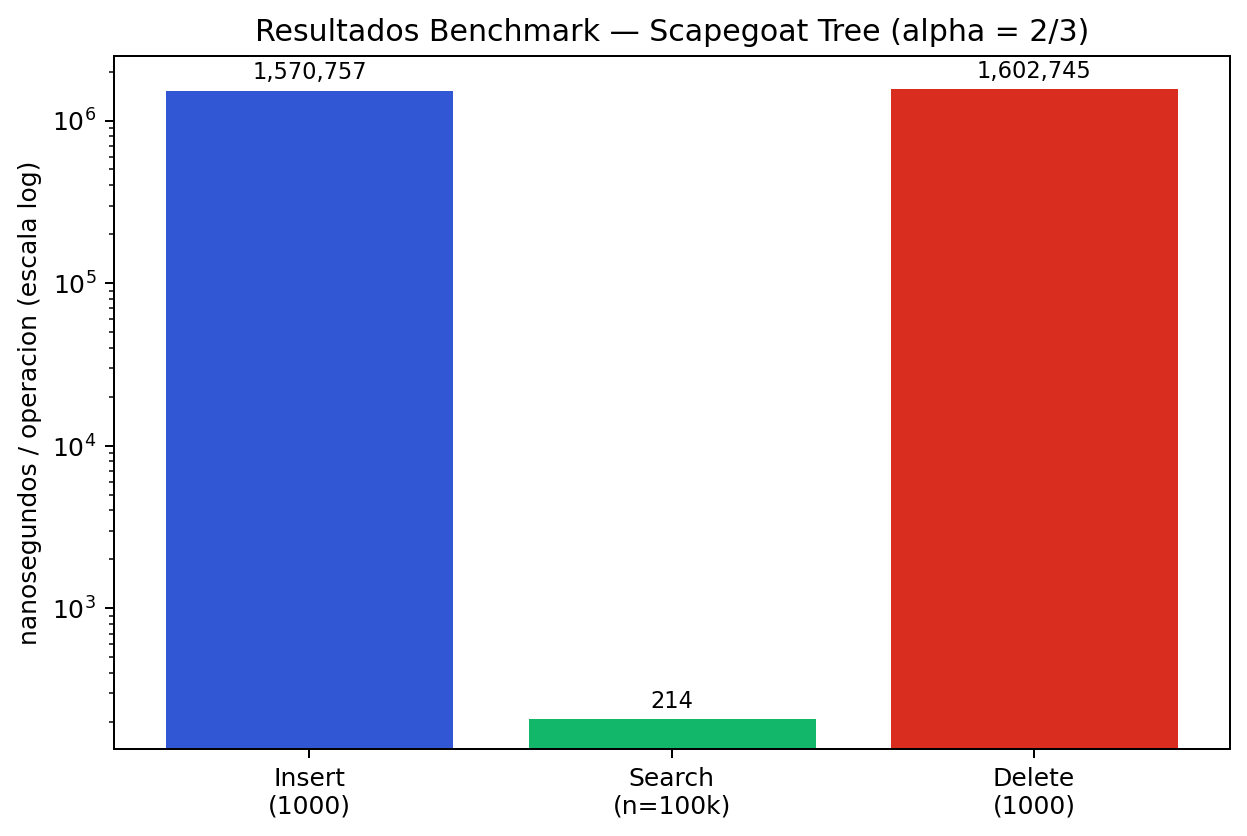
\includegraphics[width=0.78\textwidth]{diagrams/04-benchmark.png}
  \caption{Comparativa de benchmarks (escala logarítmica)}
  \label{fig:benchmark}
\end{figure}

\begin{figure}[H]
  \centering
  \begin{tikzpicture}
    \begin{axis}[
      ybar,
      bar width=18pt,
      width=12cm,
      height=7cm,
      ylabel={ns/op (escala log)},
      ymode=log,
      symbolic x coords={Insert, Search, Delete},
      xtick=data,
      ymin=100,
      ymax=10000000,
      nodes near coords={\pgfmathprintnumber\pgfplotspointmeta},
      every node near coord/.append style={font=\footnotesize, anchor=west, xshift=2pt},
      grid=major,
      grid style={dashed,gray!30},
      scaled y ticks=false
    ]
      \addplot[fill=blue!55] coordinates {(Insert,1570757) (Search,214) (Delete,1602745)};
    \end{axis}
  \end{tikzpicture}
  \caption{Gráfico de barras --- tiempos promedio por operación}
  \label{fig:benchmark-bars}
\end{figure}

\section{Interpretación}

La búsqueda exhibe $\sim 4.7 \times 10^6$ ops/s con cero asignaciones de heap. Insert y Delete muestran picos por reconstrucciones; la envolvente superior de inserción ordenada crece más rápido que en secuencias aleatorias, confirmando la teoría del scapegoat.

\chapter{Gestión del proyecto y reporte de commits}

\section{Responsabilidades por entregable}

\begin{table}[H]
  \centering
  \caption{Distribución de responsabilidades del equipo}
  \begin{tabular}{@{}lcccc@{}}
    \toprule
    \textbf{Integrante} & \textbf{E1} & \textbf{E2} & \textbf{E3} & \textbf{E4} \\
    \midrule
    [Integrante 1] & Líder & Soporte & --- & --- \\
    [Integrante 2] & Soporte & Líder & Soporte & --- \\
    [Integrante 3] & --- & Soporte & Líder & Soporte \\
    [Integrante 4] & --- & --- & Soporte & Líder \\
    \bottomrule
  \end{tabular}
\end{table}

\section{Cronograma (semanas 9--15)}

\begin{table}[H]
  \centering
  \caption{Cronograma del proyecto}
  \begin{tabular}{@{}cl@{}}
    \toprule
    \textbf{Semana} & \textbf{Hito} \\
    \midrule
    9 & Lectura del paper, diseño de structs y API \\
    10 & Implementación \texttt{insert}, \texttt{delete}, \texttt{rebuild} \\
    11 & Pruebas unitarias y benchmarks \\
    12 & Integración SQL Server \\
    13 & API REST y handlers \\
    14 & Frontend Vue y animaciones \\
    15 & Informe, ensayo de presentación \\
    \bottomrule
  \end{tabular}
\end{table}

\section{Historial de commits}

Repositorio: \url{https://github.com/Fravely/Spacegoat-tree}

\begin{table}[H]
  \centering
  \caption{Commits principales del repositorio}
  \begin{tabular}{@{}llll@{}}
    \toprule
    \textbf{Hash} & \textbf{Autor} & \textbf{Fecha} & \textbf{Mensaje} \\
    \midrule
    \texttt{5819a50} & Fravely & 2026-06-26 & Implementa Scapegoat Tree \\
    \texttt{f2153c8} & Fravely & 2026-06-26 & delete \\
    \texttt{34c2c8b} & Fravely & 2026-06-26 & Actu \\
    \texttt{b02d3d6} & 23101246-netizen & 2026-06-26 & Prueba \\
    \bottomrule
  \end{tabular}
\end{table}

El commit \texttt{5819a50} establece el núcleo algorítmico; los posteriores refinan eliminación y pruebas adicionales.

\chapter{Conclusiones y recomendaciones}

\section{Conclusiones de ingeniería}

La implementación del \Scapegoat{} en Go cumple las invariantes teóricas de Galperin y Rivest: inserciones ordenadas disparan reconstrucciones, eliminaciones masivas activan rebuild global, y 5000 operaciones aleatorias coinciden con un \texttt{map} de referencia.

La búsqueda es estable ($\sim$214~ns/op con $n=10^5$, cero allocations). La separación SQL Server / índice en RAM demostró ser arquitectónicamente sólida. La simulación Vue transformó un algoritmo abstracto en un artefacto observable.

\begin{figure}[H]
  \centering
  \begin{tikzpicture}[
    box/.style={rectangle, draw, rounded corners, align=center, font=\footnotesize, minimum width=2cm, minimum height=0.75cm},
    arrow/.style={-{Stealth[length=2mm]}, thick}
  ]
    \node[box, fill=blue!10] (u) {Usuario};
    \node[box, fill=blue!10, below=1cm of u] (b) {Navegador};
    \node[box, fill=green!10, below left=1cm and 0.5cm of b] (api) {API REST};
    \node[box, fill=green!10, below right=1cm and 0.5cm of b] (sql) {SQL Server};
    \node[box, fill=orange!12, below=1cm of api] (st) {Scapegoat Tree};
    \draw[arrow] (u) -- (b);
    \draw[arrow] (b) -- (api);
    \draw[arrow] (api) -- (st);
    \draw[arrow] (api) -- (sql);
  \end{tikzpicture}
  \caption{Vista general del sistema entregado}
  \label{fig:vista-general}
\end{figure}

\section{Limitaciones}

\begin{itemize}
  \item Dataset acotado a 8 productos semilla en la demo base.
  \item \texttt{size(u)} sin caché: cuello de botella en detección de desbalance.
  \item Sin persistencia de la forma del árbol; solo productos en SQL.
  \item Mutex global en API: no escala horizontalmente.
\end{itemize}

\section{Lecciones aprendidas}

Los punteros en Go deben reasignarse con cuidado durante \texttt{rebuild}. Las pruebas contra \texttt{map} fueron indispensables. El patrón \texttt{POST $\rightarrow$ GET /api/tree} mantiene la UI consistente, pero las animaciones requieren el snapshot previo a la mutación para mostrar caminos de búsqueda correctos.

\section{Recomendaciones futuras}

Almacenar \texttt{size} por nodo, pipeline de carga masiva con \texttt{BULK INSERT}, fuzz testing con \texttt{testing/fuzz}, y migración del frontend a Vue con Vite para producción.

\chapter*{Referencias}
\phantomsection
\addcontentsline{toc}{chapter}{Referencias}

\begin{enumerate}[label={[\arabic*]}, leftmargin=2em, itemsep=0.4em]
  \item Galperin, G. F., \& Rivest, R. L. (1993). \textit{Scapegoat trees}. Proceedings of the Fourth Annual ACM-SIAM Symposium on Discrete Algorithms (SODA), 165--174.
  \item Cormen, T. H., Leiserson, C. E., Rivest, R. L., \& Stein, C. (2009). \textit{Introduction to Algorithms} (3rd ed.). MIT Press. Capítulos 12--13.
  \item Go Project. (2024). \textit{Go Generics}. \url{https://go.dev/doc/tutorial/generics}
  \item Microsoft. (2024). \textit{SQL Server Documentation}. \url{https://learn.microsoft.com/sql/}
  \item Vue.js Project. (2024). \textit{Vue.js 3 Guide}. \url{https://vuejs.org/guide/}
\end{enumerate}

\chapter*{Anexo A --- Comandos de ejecución}
\phantomsection
\addcontentsline{toc}{chapter}{Anexo A --- Comandos de ejecución}

\begin{lstlisting}[style=gocode]
go test ./scapegoat/...
go test -bench=Benchmark -benchmem ./scapegoat/
go run ./cmd/sqlserver-demo
go run ./cmd/simulation
\end{lstlisting}

\chapter*{Anexo B --- Variables de entorno SQL Server}
\phantomsection
\addcontentsline{toc}{chapter}{Anexo B --- Variables de entorno}

\begin{lstlisting}[style=pscode]
$env:SQLSERVER_HOST="localhost"
$env:SQLSERVER_DATABASE="InventarioProductosDB"
$env:SQLSERVER_USER="sa"
$env:SQLSERVER_PASSWORD="TuPassword"
$env:SQLSERVER_ENCRYPT="disable"
$env:SQLSERVER_TRUST_CERT="true"
\end{lstlisting}

\vfill
\begin{center}
  \small\textit{Documento generado para el Trabajo Final de Algoritmos y Estructura de Datos --- Universidad ESAN --- Semestre 2026-1.}
\end{center}


\end{document}
